\subsubsection{Part 2:}

\begin{gather*}
	Throughput=\frac{rxPackets*1000*8}{txTime} \\
	TP_{1-10 Users}= 1000Kbps\\
	TP_{20 Users}= \frac{1686.45*1000*8}{20}\\
	= 647.58Kbps (\text{using average number of rxPackets}) \\
	TP_{20 Users} = 989.92Kbps (\text{using Bash Script}) \\
	TP_{50 User}= 989.92Kbps (\text{using Bash Script}) \\
\end{gather*}

\begin{figure}[H]
	\centering
	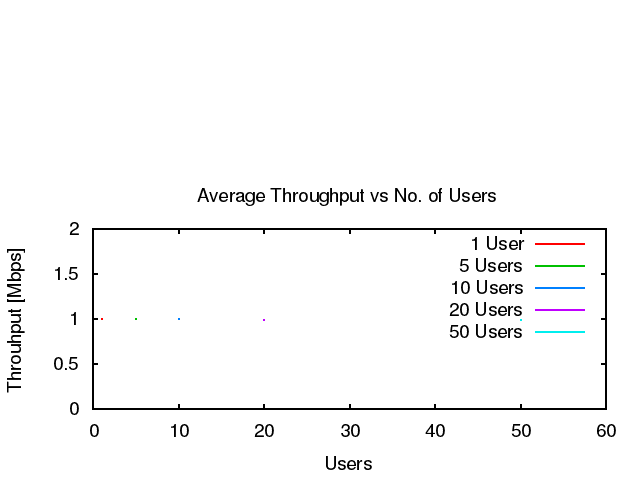
\includegraphics[width=0.8\textwidth]{images/EE500/QC/P2/Images/wifi-throughput}
	\caption{Throughput for systems with 0 to 50 users}
	\label{fig:QCP2throughput}
\end{figure}

\begin{gather*}
	\overline{delay}=\frac{delaySum}{rxPackets} \\
	\overline{delay}_{1 User}=441013ns \\
	\overline{delay}_{5 User}=2807059ns \\
	\overline{delay}_{10 User}=8420910ns \\
	\overline{delay}_{20 User}=277970000ns \\
	\overline{delay}_{50 User}=1530570000ns \\
\end{gather*}

\begin{figure}[H]
	\centering
	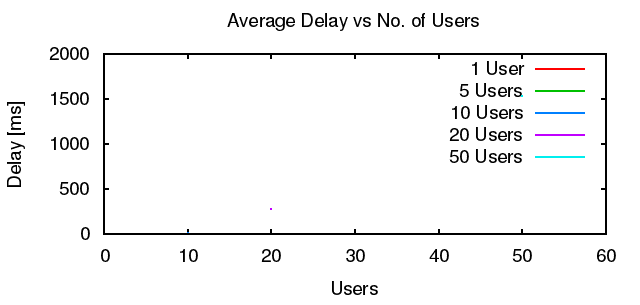
\includegraphics[width=0.8\textwidth]{images/EE500/QC/P2/Images/wifi-delay}
	\caption{Delay for systems with 0 to 50 users}
	\label{fig:QCP2delay}
\end{figure}

\begin{gather*}
	PLR=\frac{lostPackets}{rxPackets+lostPackets} \\
	PLR_{1 User}=0 \\
	PLR_{5 User}=0 \\
	PLR_{10 User}=0 \\
	PLR_{20 User}=1.08\% \\
	PLR_{50 User}=1.08\% \\
\end{gather*}

\begin{figure}[H]
	\centering
	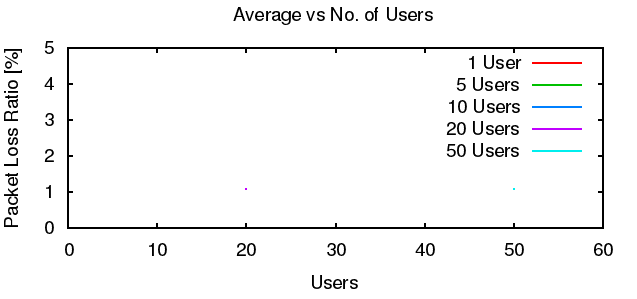
\includegraphics[width=0.8\textwidth]{images/EE500/QC/P2/Images/wifi-loss}
	\caption{Loss for systems with 0 to 50 users}
	\label{fig:QCP2loss}
\end{figure}
